%Tipo de documento
\documentclass[a4paper,12pt,twoside]{article} %book, report, letter, beamer


%Paquetes

%Configuracion inicial
\usepackage[utf8]{inputenc}
%\UseRawInputEncoding
\usepackage[spanish]{babel}

%Hipervinculos dinamicos
\usepackage[backref]{hyperref}
%Matematicas
\usepackage{amssymb}
\usepackage{amsmath}
\usepackage{amsbsy}
%Comentarios de varias lineas
\usepackage{comment}
%Insertar imagenes
\usepackage{graphicx}
\graphicspath{ {IMAGENES/} }
%Cuadros de codigo
\usepackage{listings}



% Cuerpo del documento -------------------------------------------------
%Entorno: comando especial que cuenta con parte de incio y de fin.

\begin{document}

%Portada
\begin{titlepage}
\centering

{
\includegraphics[width=0.6\textwidth]{foto_portada.png}\par}
\vspace{1cm}

{\bfseries\LARGE Escuela Técnica Superior de Ingeniería Informática y Telecomunicaciones \par}
\vspace{0.4cm}

{\scshape\Huge Algoritmos Voraces \par}
\vspace{0.4cm}

{\itshape\Large Tercera Práctica de Algorítmica \par}
\vspace{0.5cm}

{\itshape\Large Doble Grado en Ingeniería Informática y Matemáticas \par}
\vspace{0.4cm}

{\Large Autores: \par}
{\Large Elena Abreu Fernández \par}
{\Large Antonio Cantillo Molina \par}
{\Large Leandro Jorge Fernández Vega \par}
\vfill

{\Large Abril 2023 \par}

\end{titlepage}

% Crea indice
\tableofcontents
\newpage


\section{Objetivos}


	\begin{itemize}
		\item Conocer en profundidad la implementación de un algoritmo de tipo \textit{Voraz} o \textit{Greedy}.
		\item Saber demostrar la optimalidad de una solución de un algoritmo \textit{Greedy}.
		\item Abordar el diseño de heurísticas .
		\item Aprender a utilizar recursos gráficos como GNUPLOT y aplicar conocimiento estadístico a los análisis.
	\end{itemize}
\newpage


\section{Introducción}

Se plantea la elaboración de un algoritmo de tipo \textit{"Greedy"}. Estos algoritmos son no previsores, se utilizan generalmente para problemas de optimización y toman decisiones en función de la información disponible en ese momento, sin volver a replantearlas en el futuro.\\

\subsection{Características}

\begin{itemize}
    \item Se utilizan generalmente para resolver problemas de optimización: máximo o mínimo.
    \item Un algoritmo “greedy” toma las decisiones en función de la información local que está disponible en cada momento (“miopes”).
    \item Una vez tomada la decisión no se la vuelve a replantear en el futuro.
    \item Suelen ser rápidos y fáciles de implementar.
    \item No garantizan alcanzar la solución óptima.
\end{itemize}
\subsection{Elementos}

\begin{itemize}

	\item Conjunto de candidatos: posibles decisiones
	\item Conjunto de seleccionados: decisiones tomadas hasta el momento.
	\item Función solución: determina si se ha alcanzado una solución.
	\item Función de factibilidad: determina si es posible completar el conjunto de candidatos seleccionados para alcanzar una solución al problema.
	\item Función selección: determina el candidato más prometedor entre los seleccionados.
        \item Función objetivo: da el valor de la solución alcanzada.

\end{itemize}

\newpage


\subsection{Datos Técnicos del Computador Utilizado}

\begin{itemize}

	\item Nombre del dispositivo: ASUS LAPTOP-7LR09K87

	\item Procesador: 11th Gen Intel(R) Core(TM) i7-11370H @ 3.30GHz   3.30 GHz

	\item RAM instalada: 16,0 GB (15,7 GB usable)

	\item Tipo de sistema: Sistema operativo de 64 bits.

	\item Arquitectura: x86\_64

	\item Cachés: L1d: 48 KiB (1 instance), L1i: 32 KiB (1 instance), L2: 1.3 MiB (1 instance), L3: 12 MiB (1 instance)

\end{itemize}
\vspace{1cm}

\subsection{Tipos de Análisis a Realizar}

\subsubsection{Análisis Teórico}

Para determinar a qué orden de eficiencia teórico pertenece un algoritmo, consideramos las siguientes definiciones:

\begin{itemize}

	\item Caso Peor:\\
	\begin{math}
	T(n) \in O(f(n)) \Leftrightarrow \exists K \in \mathbb{R^+} , \exists n_0 \in \mathbb{N} : T(n) \leq K \cdot{f(n)} \ \ \forall n > n_0
	\end{math}
	
	\item Caso Exacto:\\
	\begin{math}	
	T(n) \in \Theta(f(n)) \Leftrightarrow \exists K \in \mathbb{R^+} , \exists n_0 \in \mathbb{N} : T(n) = K \cdot{f(n)} \ \ \forall n > n_0
	\end{math}
	
	\item Caso Mejor:\\
	\begin{math}
	T(n) \in \Omega(f(n)) \Leftrightarrow \exists K \in \mathbb{R^+} , \exists n_0 \in \mathbb{N} : T(n) \geq K \cdot{f(n)} \ \ \forall n > n_0
	\end{math}
	
\end{itemize}

\vspace{1cm}




\newpage
\subsubsection{Análisis Empírico}

El análisis empírico supone la ejecución del algoritmo de ordenación para diferentes tamaños del vector. Para ello, usaremos los siguientes recursos:\\


\begin{itemize}
	\item La biblioteca $<$chrono$>$ y sus funciones para medir tiempos.
	
	\lstset{language=C++}
	\begin{lstlisting}

#include <chrono>
	
high_resolution_clock::time_point t_antes, t_despues;
duration<double> transcurrido;

t_antes = high_resolution_clock::now();

algoritmo(a0,a1,...);

t_despues = high_resolution_clock::now();
transcurrido = 
duration_cast<duration<double>>(t_despues - t_antes);
cout << "el tiempo empleado es " 
<< transcurrido.count() << " s." << endl;
	
	\end{lstlisting}
	
\vspace{1cm}

	\item El siguiente script para automatizar la obtención de resultados para diferentes tamaños:

	\lstset{language=Bash}
	\begin{lstlisting}
#!/bin/bash 

i="inicio"
while [ "$i" -le "tope" ]
do
        generador salida.dat $i
 	algoritmo salida.dat >> salida.dat
        i=$(( $i + "salto" ))
done
      

	\end{lstlisting}
	
\end{itemize}

\newpage
\subsubsection{Análisis Híbrido}

Consiste en obtener las constantes ocultas de la función del algoritmo. Para ello, utilizamos la herramienta GNUPLOT. Pondremos como ejemplo un algoritmo cuadrático.\\

Primero deberemos introducir la ecuación de la que queremos obtener los coeficientes:\\

\fbox{gnuplot$>$ f(x) = a0*x*x+a1*x+a2}\\

Después le indicaremos a GNUPLOT que realice un ajuste por mínimos cuadrados, donde \textit{salida.dat} es el fichero de datos.\\

\fbox{gnuplot$>$ fit f(x) 'salida.dat' via a0,a1,a2}\\

La parte que más interesa es el apartado \textit{\textbf{Final set of parameters}}, donde se encuentra el valor de los parámetros.\\

Para graficar utilizamos:\\

\fbox{gnuplot$>$ 'salida.dat', f(x) title 'Curva de Ajuste'}\\

Para determinar la bondad del ajuste, podemos utilizar la varianza, aunque el propio análisis teórico y los resultados gráficos nos permiten confirmar que la ecuación parabólica y n-logarítmica representan buenas aproximaciones para los algoritmos a tratar.

\newpage


\section{Primer Problema: Codificación Textual de Imágenes}

El problema que se plantea resolver es el siguiente:\\

Una imagen se almacena como una matriz bidimensional (f × c) de píxeles. Cada píxel es codificado como un valor entero (int, representado con 64 bits). El sistema de captación utiliza una representación \textit{raw}, es decir, se almacena expresamente cada píxel, utilizando un espacio total de f × c × 8 bytes.\\

Sin embargo, hay situaciones en las que la distribución de colores de la imagen es bastante sesgada y puede ser conveniente utilizar una codificación distinta para los píxeles. De esta forma, podemos asignar a cada color de píxel un código con distinta longitud. Por simplicidad consideraremos que el código está formado únicamente por caracteres numéricos hexadecimales, es decir, {0, 1, . . . , 9, A, B, C, D, E}. Cada uno de estos símbolos se almacena usando un \textit{nible}, es decir, 4 bits. Por tanto, en cada byte se pueden almacenar 2 caracteres hexadecimales. Ejemplos de códigos a asignar serıían 0, 0A, 12C, . . . .\\

Se pide diseñar un algoritmo para, dada una imagen, encontrar una codificación de los colores presentes en la misma, tal que la representación basada en esta codificación sea lo más corta (en tamaño) posible.


\newpage

\subsection{Explicación}

Para resolver dicho problema hemos decidido recopilar en un contenedor tipo map todos los colores presentes en una imagen dada junto con las veces que se repite. A continuación, los hemos ordenado de más a menos repeticiones pues, para obtener la codificación más corta posible, la opción más óptima es asignar a los píxeles que más se repiten el código más corto.\\

\subsection{Generador de Casos}

\subsubsection{Explicación}
El término \textit{generador de casos} hace referencia a un programa que establece la situación más adecuada para trabajar.\\

Para ello, hemos implementado un programa que reciba como parámetros dos enteros que representen las dimensiones de la matriz y un dato tipo string que represente el nombre del fichero en el que vamos a volcar los datos. A continuación generamos números enteros random que representaran los píxeles de la imagen.\\

Será necesario, posteriormente, procesar los datos del fichero generado para rellenar la matriz de píxeles sobre la que utilizar el algoritmo.

\newpage

\subsubsection{Implementación}

\lstset{language=C++}
\begin{lstlisting}

#include <iostream>
#include <string>
#include <fstream>

using namespace std;

int main(int argc, char *argv[]) {

    // Comprobacion de argumentos

    if(argc != 4) exit(-1);

    // Tomamos argumentos
    string fichero=argv[1];
    int filas=stoi(argv[2]);
    int cols=stoi(argv[3]);

    ofstream salida;
    salida.open(fichero);

    // Rellenamos el fichero con los datos de la matriz
    salida << filas << " " << cols << endl;

    //Recorrer matriz y meter elem en salida
    const int TOPE_RANDOM=255;
    for (int i = 0; i < filas; i++){
        for (int j = 0; j < cols; j++) {
            salida << rand() % TOPE_RANDOM << " ";
        }
        salida << endl;
    }

    // Cerramos el fichero y lo devolvemos.
    salida.close();

    return 0;
}

\end{lstlisting}

\newpage


\subsubsection{Implementación}

\lstset{language=C++}
\begin{lstlisting}
/*
* struct que encapsula el concepto de color a nivel de imagen.
* @field pixel Entero que representa el valor de pixel.
* @field reps Cantidad de veces que esta el color presente
* en la imagen.
* @field cod Codigo asignado a cada pixel tras realizar 
* una codificacion.
*/
struct color{
    int pixel;
    int reps;
    string cod;
};
	
/*
* Funcion que convierte un entero decimal a hexadecimal.
* @param n Numero a convertir.
* @return Numero hexadecimal en forma de cadena de caracteres.
*/
string Hexadecimal(int n) { //O(log(n))
    stringstream stream;
    stream << hex << n;
    return stream.str();
}

/*
* Criterio de ordenacion para el algoritmo sort. Servira para 
ordenar un vector tipo pair<int,int>.
* @param p1,p2 Parejas a comparar.
*/
bool ordenaReps (const pair<int,int>& p1, const pair<int,int>& p2){

    return p1.second > p2.second;
}





/*
* Prepara el conjunto de candidatos a utilizar en el algoritmo voraz.
* @param matriz Matriz de pixeles que representa una imagen.
* @param f Numero de filas de la matriz.
* @param c Numero de columnas de la matriz.
* @return El conjunto de candidatos como vector, ordenado 
por repeticiones de cada color.
*/
vector<pair<int,int>> Prepara_Candidatos(vector<vector<int>> matriz,
                                        int f, int c){

    map<int,int> candidatos;
    //O((f*c)*log(f*c))
    for (int i=0; i < f; i++) {
        for (int j = 0; j < c; j++) {
        
            //O(log(f*c))
            if(!candidatos.insert
                (pair<int,int>(matriz[i][j],1)).second){
                candidatos[matriz[i][j]]++;
            }
            //Almacenamos todos los colores presentes en la imagen 
            //junto con las veces que se repiten, sera nuestro
            //conjunto de candidatos
        }
    }
    
    //Ordenamos los candidatos de mas a menos repeticiones 
    //en la imagen

    vector<pair<int,int>> candidatos_ord
    (candidatos.begin(),candidatos.end());
    sort(candidatos_ord.begin(),candidatos_ord.end(), ordenaReps);

    return candidatos_ord;
}





/*
* Algoritmo voraz que proporciona una codificacion para 
* una imagen con el objetivo de reducir su tamano de 
* almacenamiento.
* @param matriz Matriz de pixeles que representa una imagen.
* @param f Numero de filas de la matriz.
* @param c Numero de columnas de la matriz.
* @return Objeto tipo pair que almacena un vector con la 
* codificacion y el nuevo tamanio segun esta codificacion.
*/
pair<vector<color>,int> Voraz(vector<vector<int>> matriz,
                                int f, int c) {

    //Obtenemos el conjunto de candidatos con las 
    //especificaciones necesarias.
    
    //O((f*c)*log(f*c))
    vector <pair<int,int>> candidatos_ord= 
                    Prepara_Candidatos(matriz,f,c);
    

    //Una vez ordenado, procedemos a asignar la codificacion 
    //correspondiente: asignamos los numeros que ocupen menos
    //bytes a los pixeles que mas se repitan

    //Calculamos el tamano de nuestra nueva codificacion
    vector<color> seleccionados;
    int tamanio=0;

    //O(log((f*c)!)) = O((f*c)*log(f*c))
    for(int i=0; i<candidatos_ord.size(); ++i) {
        color seleccionado;
        seleccionado.pixel = candidatos_ord[i].first;
        //O(log(i))
        seleccionado.cod=Hexadecimal(i); 
        seleccionado.reps=candidatos_ord[i].second;

        seleccionados.push_back(seleccionado);
        tamanio+=
        (seleccionados[i].cod.length()*seleccionados[i].reps);
        //Funcion objetivo
    }

    return pair<vector<color>,int>(seleccionados,tamanio);
}
\end{lstlisting}
\vspace{1cm}

\subsection{Demostración de Validez}

A continuación, demostramos que el algoritmo escogido para dar con la solución de nuestro problema es el más óptimo.\\

Tenemos un vector en el que almacenamos la codificación que se asigna a cada color de una imagen. En nuestra solución ordenamos el vector de colores de más menos repeticiones, de manera que:\\

$\sum_{i=0}^{n-1} l_i \cdot{r_i}$ es la longitud total de la codificación, donde $li$ la longitud de la codificación del color $i$, y $ri$ es el número de veces que se repite el color $i$.\\

Para probar que la solución es óptima, suponemos por reducción al absurdo que existe otra codificación que cumple:\\
\\
$\sum_{i=0}^{n-1} l'_i*r'_i < \sum_{i=0}^{n-1} l_i \cdot{r_i} $ , donde $l'_i, r'_i,  \forall i \in \{0,1,...n-1\}$ son la longitud y repeticiones asociadas a la nueva codificación.\\

Como en esta solución no se ordenan los colores por repeticiones, nos encontramos con el caso de que un color que se encontraba en la posición $i$ pasa a la posición $j$ con la nueva codificación, de manera que su longitud puede verse modificada. Así, en el caso de que $i<j$, como las repeticiones no cambian y las codificaciones se asignan en orden creciente, es decir, primero se asignan las codificaciones más cortas, tenemos que:\\

$l'_j \cdot {r'_j} > l_i \cdot {r_i}$, y, teniendo en cuenta que las repeticiones son las mismas en ambos casos, obtenemos $l'_j>l_i$. Esto es contradictorio, pues el tamaño aumenta, lo que no tiene sentido si la nueva codificación es más óptima.\\

Así, queda demostrado que la solución seleccionada es la óptima.



\newpage

\subsection{Análisis de Eficiencia}

\subsubsection{Análisis Teórico}

Claramente $T_{Voraz}(f,c) \in O(f \cdot{c} \log{f \cdot{c}})$, pues:\\

Analizando la función Prepara\_Candidatos, los bucles anidados realizarán $f \cdot {c} $ iteraciones de una operación de inserción en un mapa, que es logarítmica.

En la función Voraz, tendremos una llamada a Prepara\_Candidatos de orden $O((f \cdot {c}) \log{(f \cdot{c})})$. 


A continuación, hay que tener en cuenta que en el bucle se llama a la función Hexadecimal, que tiene una eficiencia de $O(\log{n})$, donde $n$ es el número entero al que se le calcula su valor hexadecimal. Haciendo la respectiva sumatoria:\\

Llamando a $f \cdot c=n$\\

$\sum_{i=1}^{n} \log{(i)} =
\log{(\prod_{i=1}^{n} {i})} = \log{(n!)} = \log{((f \cdot{c})!)}$\\

Teniendo en cuenta la conocida como \textit{Fórmula de Stirling}, que enuncia la siguiente aproximación para $n$ suficientemente grandes: $\log{n!} \approx n\log{n} - n$\\

Por tanto, el bucle tendrá una eficiencia de $O((f \cdot {c}) \log{(f \cdot{c})})$.\\

Finalmente, concluimos que $T_{Voraz}(f,c) \in O((f\cdot{c}) \log{(f\cdot{c})})$


\newpage
\subsubsection{Análisis Empírico}

\begin{table}[h]
	\begin{center}
		\begin{tabular}{|c|c|}
		\hline
		Tamaño & Tiempo \\
		\hline
		500 & 0.0296728 \\
		1000 & 0.091241 \\
		1500 & 0.20113 \\
		2000 & 0.355693 \\
		2500 & 0.558893 \\
		3000 & 0.83031 \\
		3500 & 1.18843 \\
		4000 & 1.4311 \\
		4500 & 1.71356 \\
		5000 & 2.06774 \\
		5500 & 2.72843 \\
		6000 & 4.6062 \\
		6500 & 4.9699 \\
		7000 & 4.51009 \\
		7500 & 5.04839 \\
		8000 & 5.81591 \\
		8500 & 6.61049 \\
		9000 & 7.51259 \\
		9500 & 8.61772 \\
		10000 & 9.13311 \\
		10500 & 10.0056 \\
		11000 & 11.0392 \\
		11500 & 12.0955 \\
		12000 & 12.8952 \\
		12500 & 14.0145 \\
		\hline
		\end{tabular}
	\end{center}
	\caption{Algoritmo Voraz}
\end{table}

\newpage


\subsubsection{Análisis Híbrido}

\begin{figure}[h]
  \begin{center}
  
  	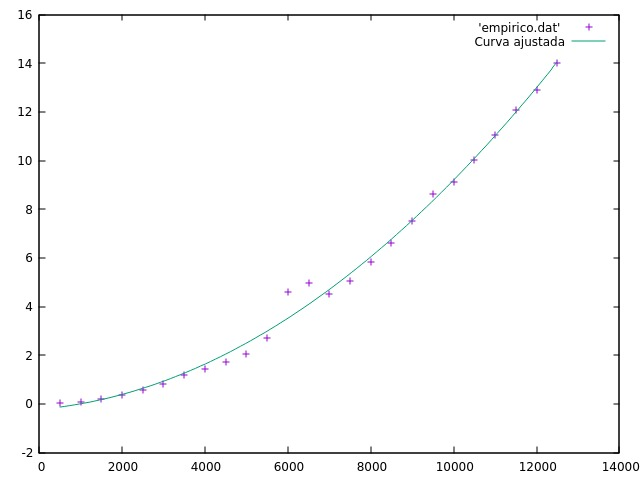
\includegraphics[scale=0.7]{IMAGENES/ajustehibrido.jpeg}
  	\caption{Algoritmo ajustado.}
  	
  \end{center}
\end{figure}


El análisis teórico nos permite comprobar que la curva de ajuste es una parábola de ecuación:\\

$T(n) = 7.96736 \cdot{10^{-8}} n^2 +0.000145488\cdot \log{(n^2)}$\\

con una varianza residual $Var_{res} =0.124005$, con lo cual es fiable el ajuste.

\newpage

\section{Segundo Problema: El viajante de comercio (PVC)}

Una empresa que comercializa componentes informáticos ha contratado un nuevo comercial. Al agente le ha asignado un conjunto de clientes, facilitándole la información relevante de cada uno, que incluye nombre, correo electrónico, teléfono y dirección postal. El director comercial le encarga al nuevo agente visitar a todos esos clientes, con el objetivo de hacer buenas ventas y que no vuelva hasta que haya visitado a todos los clientes. Por tanto, el recorrido considerado debe comenzar y finalizar en la empresa. Además, sólo podrá visitar cada cliente una sola vez. Además, para reducir gastos de desplazamiento, la distancia total recorrida debe ser lo más corta posible.


\paragraph{Aclaración}
Este problema es de tipo NP-completo, lo que quiere decir que no se ha encontrado un algoritmo que encuentre la solución óptima en tiempo polinomial para instancias grandes del problema. Por esta razón, se recurre a heurísticas para encontrar soluciones aceptables al problema. Se nos pide desarrollar tres heurísticas distintas para la solución de este problema.\\

Estas tres heurísticas proponen como solución un Ciclo \textit{Hamiltoniano}, en el cual se pasa una única vez por cada vértice. Sin embargo, no podemos determinar si este ciclo es la solución óptima, en cada caso.

Para ello, hemos usado la siguiente implementación:\\

\lstset{language=C++}
\begin{lstlisting}
/*
 * struct que encapsula el concepto de cliente de un 
   vendedor cualquiera.
 * @field x Coordenada x del cliente.
 * @field y Coordenada y del cliente.
 * @field id Identificador del cliente.
 */
struct cliente{
    double x;
    double y;
    int id;

    bool operator < (cliente cliente) const{
        return id<cliente.id;
    }
};


\end{lstlisting}
\newpage

\subsection{Generador-PVC}
\lstset{language=C++}
\begin{lstlisting}
#include <iostream>
#include <string>
#include <fstream>
#include <random>

using namespace std;

int main(int argc, char *argv[]) {

    // Comprobacion de argumentos
    if (argc != 3) exit(-1);

    // Tomamos argumentos
    string fichero = argv[1];
    int n_clientes = stoi(argv[2]);

    ofstream salida;
    salida.open(fichero);

    // Rellenamos el fichero con los datos de los clientes
    salida << n_clientes << endl;

    // Generar clientes con sus identificadores 
    // y coordenadas x e y.
    const int MIN=0, MAX=10;
    std::random_device rd;
    std::default_random_engine eng(rd());
    std::uniform_real_distribution<double> distr(MIN,MAX);

    for (int i = 0; i < n_clientes; i++) {
        salida << i << " " << distr(eng) << " " 
               << distr(eng) << endl;
    }

    // Cerramos el fichero y lo devolvemos.
    salida.close();
    return 0;
}

\end{lstlisting}


\subsection{Primera Heurística}

\lstset{language=C++}
\begin{lstlisting}
/*
*Funcion que crea una matriz que almacena todas las distancias 
*entre todos los clientes entre si.
*La posicion [i][j] guarda la distancia entre el cliente i y el j
*@param clientes Vector de clientes.
*@return Matriz de todas las distancias.
*/
vector<vector<double>> matriz_dist(vector<cliente> clientes){
    vector<vector<double>> matriz(clientes.size(),
                vector<double> clientes.size()));
    for(int i=0; i<clientes.size(); ++i){
        for(int j=0; j<clientes.size(); ++j){
            matriz[i][j] = distancia(clientes[i],clientes[j]);
        }
    }
    return matriz;
}

/*
*Devuelve el minimo elemento de una fila.
*@param fila Fila de la que se extrae el minimo.
*@param id
*/

int min_fila(vector<double> fila, int id){
    int pos_min = 0;
    while((fila[pos_min]==0 || fila[pos_min]==-1) && pos_min 
    <fila.size()) 
    pos_min++;

    double minimo = fila[pos_min];
    for(int i = pos_min;i<fila.size();++i){
        if(fila[i] < minimo && i!=id && fila[i]!=-1){
            minimo = fila[i];
            pos_min = i;
        }
    }
    return pos_min;
}

/*
*Funcion auxiliar que borra de la matriz las distancias 
*relacionadas con los clientes que ya hayan sido seleccionados.
*El borrado se realiza poniendo los elementos a borrar a -1.
*@param matriz Matriz de la que borrar.
*@param pos Fila y columna que borrar.
*/
void borrar_matriz(vector<vector<double>> &matriz, int pos){
    for(int i=0 ; i<matriz.size();i++) {
        matriz[pos][i]=-1;
        matriz[i][pos]=-1;
    }
}

/*
*Heuristica del Problema del Viajante de Comercio que 
*calcula la ruta mas optima para visitar a todos los clientes.
*@param candidatos Vector de clientes a visitar.
*@return Vector de clientes que representa la ruta mas 
*optima a realizar.
*/

vector<cliente> Alg_PVC1(vector<cliente> candidatos){

    vector<cliente> seleccionados;
    vector<vector<double>> matriz=matriz_dist(candidatos);
    int n = candidatos.size();

    int i=0;

    while(seleccionados.size()<n){ 
    //Hasta que se hayan visitado todos los clientes

        //Se selecciona el cliente mas cercano
        seleccionados.push_back(candidatos[i]);

        int siguiente = min_fila(matriz[i],i);
        borrar_matriz(matriz,i); 

        
        //Se eliminan los clientes visitados porque no podemos 
        //visitar dos veces al mismo
        
        i=siguiente;
    }
    seleccionados.push_back(candidatos[0]);

    return seleccionados;
}



\end{lstlisting}

\vspace{1cm}
\subsubsection{Justificación}
Esta primera heurística es conocida como "la del vecino más cercano", y consiste en comenzar la ruta en una ciudad aleatoria y a continuación ir desplazándose a la más cercana desde ahí. Así, podemos afirmar que va a ir seleccionando la ruta más corta posible en todo momento, aunque no para todos los tamaños del problema se podrá conseguir la solución óptima.
\newpage


\subsection{Segunda Heurística}

\lstset{language=C++}
\begin{lstlisting}
/*
 * Funcion que calcula la posicion mas optima en la que
   insertar el siguiente cliente a visitar.
 * @param ruta Vector de clientes que se han seleccionado.
 * @param siguiente Cliente a insertar.
 * @return Posicion mas optima donde meter @cliente.
*/
int pos_optima(vector<cliente> ruta, cliente siguiente){
    double min = INFINITY;
    int pos_optima = 0;
    for (int i = 1; i < ruta.size(); ++i) {

        double distancia_izq = 
        distancia(siguiente, ruta[i-1]);
        double distancia_dcha = 
        distancia(siguiente, ruta[i]);

        //Calculamos la distancia que ahorrariamos si
        //incluimos el siguiente cliente entre i e i-1
        double distancia_ahorro = 
        distancia(ruta[i-1], ruta[i]) - distancia_izq -
        distancia_dcha;
        double distancia_total = 0;

        for (int j = 0; j < ruta.size() - 1; j++) {
            distancia_total += distancia(ruta[j], ruta[j+1]);
        }
        distancia_total += distancia_ahorro;
        if (distancia_total <min) {
            min = distancia_total;
            pos_optima = i;
        }
    }
    return pos_optima;
}






/*
 * Funcion que devuelve la posicion del siguiente a insertar. 
 Es decir, el mas cercano.
 * @param clientes Vector de clientes a visitar (candidatos).
 * @param actual Posicion del cliente recien insertado.
 */
int pos_min(vector<cliente> clientes, int actual){
    int pos=0;
    double min = distancia(clientes[pos],clientes[actual]);
    for(int i=1;i<clientes.size();++i){
        if(distancia(clientes[i],clientes[actual]) < min 
        && i!=actual){
            pos = i;
        }
    }
    return pos;
}

/*
 * Heuristica del Problema del Viajante de Comercio que 
 calcula la ruta mas optima para visitar a todos los clientes.
 * @param candidatos Vector de clientes a visitar.
 * @return Vector de clientes que representa la ruta mas optima.
 */
vector<cliente> Alg_PVC2(vector<cliente> candidatos) {

    vector<cliente> seleccionados;

    //Comenzamos en una ciudad aleatoria
    srand(time(NULL));
    int pos = rand() % candidatos.size();

    cliente cliente_seleccionado = candidatos[pos];

    int siguiente;
    int pos_insercion;
    seleccionados.push_back(cliente_seleccionado);




    while(candidatos.size()!=1){
        siguiente = pos_min(candidatos,pos);
        cliente_seleccionado=candidatos[siguiente];
        pos_insercion = 
        pos_optima(seleccionados,cliente_seleccionado);
        seleccionados.insert(seleccionados.begin()+pos_insercion,
                            cliente_seleccionado);
        pos=siguiente;
        candidatos.erase(candidatos.begin()+pos);
    }
    
     //Insertamos camino de vuelta al primero.
    cliente inicial = seleccionados[0];

    seleccionados.push_back(inicial);

    return seleccionados;
}


\end{lstlisting}
\vspace{1cm}

\subsubsection{Justificación}
Como segunda heurística para resolver el problema hemos utilizado un algoritmo de inserción: siguiendo un esquema similar al de la sección anterior, tras seleccionar una primera ciudad aleatoria para nuestra ruta, elegimos la más cercana como siguiente seleccionada, antes calculando si la ruta será más corta insertándola antes o después de las ciudades ya seleccionadas. Así, con incluso más comprobaciones que en el algoritmo anterior, vamos seleccionando la ruta más corta posible. No obstante, no siempre la solución es óptima.
\newpage
\subsection{Tercera Heurística}


\begin{lstlisting}
/*
 * struct que encapsula el concepto de arista que une dos 
 * clientes.
 * @field cliente1, cliente2 Clientes unidos por la arista.
 * @field dist Distancia entre los clientes o modulo de la arista.
 */

struct arista{
    cliente cliente1;
    cliente cliente2;
    double dist ;

    /*
     * Sobrecarga del operador <
     */

    bool operator < (arista arista) const{
        return dist > arista.dist;
    }
};

/*
 * Funcion que genera un conjunto de componentes conexas 
 * con un elemento cada una.
 * @param cl Vector de clientes a partir del cual contruir 
 * el conjunto de conjuntos.
 */

set<set<cliente>> genera_Set (const vector<cliente>& cl){

    set<set<cliente>> set_clientes;

    for(int i=0; i<cl.size();i++) {
        set<cliente> c;
        c.insert(cl[i]);
        set_clientes.insert(c);
    }
    return set_clientes;
}

/*
 * Funcion que devuelve la componente conexa donde esta un
 determinado cliente.
 * @param conjunto Conjunto de conjuntos entre los que buscar
 la componente conexa.
 * @param cl Cliente que buscar entre los elementos de @conjunto.
 */

set<cliente> encuentra_Componente(set<set<cliente>> conjunto, 
                                    cliente cl){
    set<cliente> componente;

    for (set<set<cliente>>::iterator i=conjunto.begin(); 
        i!=conjunto.end(); ++i){
        set<cliente>::iterator posible=(*i).find(cl);
        if (posible!=(*i).end()) componente = *i;
    }
    return componente;
}

/*
 * Funcion quedetermina si dos conjuntos son iguales.
 * @param c1,c2 Sets a comparar.
 */

bool conjuntos_Iguales(set<cliente> c1, set<cliente> c2){

    bool iguales=false;
    if (c1.size()== c2.size()){
        iguales=true;
        for(set<cliente>::iterator i=c1.begin(); i!=c1.end() 
        && iguales;++i) {
        
            set<cliente>::iterator j=c2.find(*i);
            if (j==c2.end()) iguales=false;
        }

    }
    return iguales;
}
/*
 * Funcion que comprueba si un cliente tiene dos aristas 
 * asociadas.
 * @param clientes Vector que almacena el numero de aristas 
 * que tiene asociadas cada cliente.
 * @arista Arista de la que obtener cada cliente.
 * @return true si ambos clientes que une una arista tienen 
 * 2 aristas.
 */

bool DosVisitas(vector<int> clientes, arista arista){

    bool visitado=false;

    if(clientes.at(arista.cliente1.id)==2 ||
        clientes.at(arista.cliente2.id)==2) 
        visitado = true;

    return visitado;

}

/*
 * Funcion que une dos sets.
 * @param c1,c2 Conjuntos a unir.
 */

set<cliente> Unir (const set<cliente>& c1, 
                    const set<cliente>& c2){

    set<cliente> unir(c1);
    for (set<cliente>::iterator i=c2.begin(); i!=c2.end(); ++i)
        unir.insert(*i);
    return unir;
}






/*
 * Heuristica del Problema del Viajante de Comercio que calcula 
 * la ruta mas optima para visitar a todos los clientes.
 * @param candidatos Vector de clientes a visitar.
 * @return Vector de clientes que representa 
 * la ruta mas optima a realizar.
 */
vector<arista> Alg_PVC3(vector<cliente> candidatos) {
    vector<arista> seleccionados;
    //vector<cliente> seleccionados;
    set<set<cliente>> conjunto = genera_Set(candidatos);
    vector<arista> grafo = conjunto_aristas(candidatos);

    // Ordenamos aristas
    sort(grafo.begin(),grafo.end()); 

    //Vector que almacena cuantas aristas unen dos clientes.

    vector<int> repeticiones;
    for (int i=0; i<candidatos.size(); i++)
    repeticiones.push_back(0);

    //Ahora mismo tenemos todas las aristas ordenadas de menor
    //a mayor

    arista next = grafo.back();
    grafo.pop_back();
   // seleccionados.push_back(next);

    while (!grafo.empty() 
            && (seleccionados.size() < candidatos.size()-1)) {

        set<cliente> compu, compv;
        compu = encuentra_Componente(conjunto,next.cliente1);
        compv = encuentra_Componente(conjunto,next.cliente2);

        if(!conjuntos_Iguales(compu,compv) &&
        !DosVisitas(repeticiones,next)){

            set<cliente> unir;
            unir = Unir(compu,compv);

                //Insertamos union
                conjunto.insert(unir);
    
                //Actualizamos repeticiones
                repeticiones.at(next.cliente1.id)++;
                repeticiones.at(next.cliente2.id)++;
    
                //Borramos
                conjunto.erase(compu);
                conjunto.erase(compv);
    
                //Metemos el vertice en el conjunto de seleccionados
                seleccionados.push_back(next);
        }
        next=grafo.back();
        grafo.pop_back();
    }

    //Insertamos el camino al primer elemento.
    cliente inicio,final;
    int cont=0;
    arista ult;
    for (int i=0; i<repeticiones.size(); i++){

        if (repeticiones[i]==1){
            if(cont==0){
                inicio = candidatos[i];
                cont++;
            }
            else {
                final = candidatos[i];
            }
        }
    }
    ult.cliente1=inicio;
    ult.cliente2=final;
    seleccionados.push_back(ult);

    return seleccionados;
}

\end{lstlisting}
\newpage

\subsubsection{Justificación}
Para la última heurística nos hemos basado en el algoritmo de Kruskal como método de resolución del PVC. Así, hemos creado un tipo de dato arista, representando los caminos que unen dos clientes o vértices e implementamos un programa que va seleccionando las aristas más cortas, asegurándose de que los clientes no hayan sido visitados antes. Así, seleccionamos el camino más corto posible, aunque no podemos asegurar que siempre sea la solución óptima.

\newpage

\subsection{Análisis Comparativo}

En esta sección determinaremos cuál es la heurística más eficiente mediante la comparación de las gráficas de todas ellas.

\begin{figure}[h]
  \begin{center}
  
  	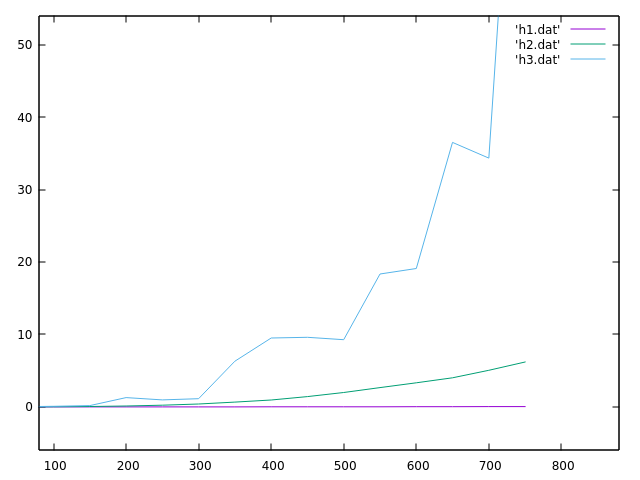
\includegraphics[scale=0.7]{IMAGENES/comparativa_h.png}
  	\caption{Comparación Heurísticas}
  	
  \end{center}
\end{figure}

Así, observamos que, para un rango de 800 clientes a visitar, el algoritmo de Kruskal rápidamente se dispara y deja de ser eficiente para tamaños pequeños. Además, es fácil concluir que, para estas magnitudes, lo más idílico es resolver el problema con la heurística del vecino más cercano, pues nos proporciona el menor tiempo de ejecución.

\newpage

\section{Conclusiones} 

\begin{itemize}
	\item La importancia del uso de algoritmos voraces para abordar problemas en los que la resolución por fuerza bruta es muy compleja.
	\item La versatilidad que ofrece la técnica \textit{Greedy} para la resolución de problemas.
	\item La necesidad de plantear distintas heurísticas para un mismo problema hasta conseguir la que nos proporcione una mejor eficiencia.
	\item La variación que puede existir entre los cálculos teóricos y empíricos debido a las características de cada dispositivo y el grado de precisión que, en cada circusntancia, es posible tomar.
	

\end{itemize}



\end{document}